\documentclass[sigconf]{acmart}
\usepackage[utf8]{inputenc}

\settopmatter{printacmref=false}
\renewcommand\footnotetextcopyrightpermission[1]{} % removes footnote with conference information in first column
\pagestyle{plain}

\usepackage{url}
\usepackage{hyperref}
\hypersetup{
    colorlinks=true,
    linkcolor=blue,
    filecolor=magenta,      
    urlcolor=cyan,
}
\urlstyle{same}


\usepackage{listings}
\usepackage{lipsum}

% Enabling Javascript syntax highlight in code snippet - BEGIN 
% https://tex.stackexchange.com/questions/89574/language-option-supported-in-listings
\usepackage{color}
\definecolor{lightgray}{rgb}{.9,.9,.9}
\definecolor{darkgray}{rgb}{.4,.4,.4}
\definecolor{purple}{rgb}{0.65, 0.12, 0.82}
\definecolor{darkgreen}{rgb}{0, .64, 0}

\lstdefinelanguage{JavaScript}{
  keywords={typeof, new, true, false, catch, function, return, null, catch, switch, var, if, in, while, do, else, case, break},
  keywordstyle=\color{blue}\bfseries,
  ndkeywords={class, export, boolean, throw, implements, import, this},
  ndkeywordstyle=\color{darkgray}\bfseries,
  identifierstyle=\color{black},
  sensitive=false,
  comment=[l]{//},
  morecomment=[s]{/*}{*/},
  commentstyle=\color{purple}\^amily,
  stringstyle=\color{darkgreen}\ttfamily,
  morestring=[b]',
  morestring=[b]"
}

\lstset{
   extendedchars=true,
   basicstyle=\footnotesize\ttfamily,
   showstringspaces=false,
   showspaces=false,
   tabsize=2,
   breaklines=true,
   showtabs=false,
   captionpos=b,
   frame=single,
   xleftmargin=0.5em,
   belowcaptionskip=0em
}

\setlength{\belowcaptionskip}{-1em}
% Enabling Javascript syntax highlight in code snippet - END

\newcommand{\APIName}{Successorships }
\newcommand{\APINameNoSpace}{Successorships}

\newcommand{\APIshort}{Shippy }
\newcommand{\rpm}{\raisebox{.2ex}{$\scriptstyle\pm$}}

\newcommand{\accessed}{accessed 2017-12-11}

\usepackage{array}
\newcolumntype{L}[1]{>{\raggedright\let\newline\\\arraybackslash\hspace{0pt}}m{#1}}
\newcolumntype{C}[1]{>{\centering\let\newline\\\arraybackslash\hspace{0pt}}m{#1}}
\newcolumntype{R}[1]{>{\raggedleft\let\newline\\\arraybackslash\hspace{0pt}}m{#1}}


\graphicspath{{figures/}{pictures/}{images/}{./}}

%opening
\title{Successorships - Fault-tolerant local WebApps}

\author{Arthur Marques \qquad Felix Grund \qquad Paul Cernek}
\affiliation{
    \institution{University of British Columbia}
    \city{Vancouver} 
    \state{BC} 
  }

\begin{document}

\begin{abstract}
As networking capabilities become more ubiquitous across different types of devices, applications that communicate over local area networks are becoming increasingly common.
This trend has been accelerated by the adoption of zero-configuration (zeroconf) networking standards that eliminate the burden of setup procedures.
Applications operating in zeroconf settings often face the challenge of maintaining reliability and consistency in the face of wireless links and mobile devices, resulting in potentially intermittent connectivity between hosts.
Fault-tolerance is thus a desirable property for such applications, but it can be difficult to achieve in practice.
To this end, we introduce Successorships, a JavaScript library that provides the appealing qualities of zeroconf enriched with fault-tolerance, to applications running in the browser.
Our library enables graceful recovery after server failure by handing over the server role to one of the clients currently in the network.
We evaluate our approach with a sample application, focusing on usage scenarios that involve interactions between users walking in and out of a single room. 
We find that our library recovers from failures gracefully after an average of 20 seconds, and that application state is maintained with eventual consistency.
\end{abstract}

\maketitle

\section{Introduction}
\label{sec:introduction}

\section{Background}
\label{sec:background}

In this section, we detail the underlying concepts that are related to our project proposal.

\subsection{Zero-configuration Networks}
\label{sec:zeroconf}



Zero-configuration networking is a combination of protocols that aims to automatically discover computers or peripherals in a network without any central servers or human administration. To do so, Zero-configuration networks have two major components that provide {\it (i)} the automatic assignment of IP addresses and host naming (mDNS), and {\it (ii)} service discovery (DNS-SD).


Roughly, when a device enters the local network, he assigns and IP/name to himself and then multicast that to the local network, resolving any name conflict that may occur in such process. IP assignment considers the link-local domain address, which draws addresses from the IPv4 169.254/16 prefix and, once an IP is selected, a host name with the suffix ``.local'' is mapped to that IP~\cite{rfc6762}. As devices are mapped to IPs/host names, their available services are discovered using a a combination of DNS PTR, SRV, and TXT records~\cite{rfc6763}, thus their services can be requested by other devices. 




\subsection{Local-area frameworks}
\label{sec:flyweb}

FlyWeb is a Web API developed by the Mozilla Firefox community which enables clients of Web applications to publish a local server from within the browser. Building on the concept of zero-configuration networks and its mDNS/DNS-SD protocols~\cite{rfc6762, rfc6763}, the server advertises itself in the local network and can be discovered by other devices which become clients to the server by connecting via a HTTP or WebSocket connection. This essentially enables cross-device communication within a local-area network.

Google Nearby Connections\footnote{\url{https://developers.google.com/nearby/connections/overview}} is a peer-to-peer networking API that allows apps to discover, connect and exchange data to other devices in a local area network. The Nearby Connections app work through a combination of Bluetooth, BLE, and Wifi hotspots in order to exchange data. However, the API does not provide details about protocols and how devices are resolved.

Opera Unite\footnote{\url{http://www.operasoftware.com/press/releases/general/opera-unite-reinvents-the-web}} also has a technology that starts a local server in the Opera browser. Their technology allows file sharing, photo sharing, and other features but, similar to Google Nearby Connections, their documentation does not clearly specify which technologies are used.

\subsection{Replication}
\label{sec:replication}

Fault tolerance and reliability in distributed systems with client-server architecture are generally achieved by data replication: information is shared on redundant server replicas such that any replica can become the new master if the current master fails. While improving system artifacts like fault-tolerance, reliability and availability, replication can come at the cost of performance: depending on the required operations in the system for replication, system performance can suffer significant bottlenecks. Different models of replication have been proposed to trade consistency for performance, resulting in different levels of consistency as a design choice for the target system. Traditionally, two strategies of replication are distinguished: \textit{active replication} and \textit{passive replication}. A third type of replication, \textit{lazy replication}, was later introduced and is gaining more attention recently. The following paragraphs describe these three types of replication.

\textbf{Active replication.} The first strategy (also called \textit{primary-backup} or \textit{master-slave}), requests to the master replica are processed to all other replicas. Given the same initial state and request sequence, all replicas will produce the same response sequence and reach the same final state. Active replication has become most prominent with the introduction of the State Machine Replication model which was introduced in the 1980s \cite{Lamport:1984} and later refined in \cite{Schneider:1990}. It is based on the concept of distributed consensus with the goal of reliably reaching a stable state of the system in the presence of failures. While providing small recovery delay after failures due to an imposed total order of state updates, computation performance can suffer tremendous bottlenecks since updates must be sequentially propagated through all replicas. 

\textbf{Passive replication.} The second strategy (also called \textit{multi-primary} or \textit{multi-master} scheme) relaxes sequential ordering: clients communicate with a master replica and updates are forwarded to backup replicas. Computation performance is improved with this pattern since all computation takes place on the master replica and only the results are propagated. The downside of the approach is that more network bandwidth is required if updates are large. Since the primary replica represents a single point of entry to clients with this approach, there must be some kind of distributed concurrency control in order to reliably restore state when the primary fails. This makes the implementation of this approach more complex and recovery potentially slower.

\textbf{Lazy replication.} A third strategy of replication was proposed in 1990: \textit{lazy replication} \cite{Ladin:1990,Ladin:1992} (also called \textit{optimistic replication}) aims at providing highest possible performance and availability by sacrificing consistency significantly. With this approach, replicas periodically exchange information, tolerating out-of-sync periods but guarantee to catch up eventually. While the traditional approaches guarantee from the beginning that all replicas have the exact same state at any point in time, lazy replication allows states to diverge on replicas, but guarantees that the states converge when the system quiesces for some time period. In contrast to the strong consistency models used in the traditional approaches, lazy replication is based on eventual consistency which has gained more attention recently, in particular in online editing platforms, NoSQL cloud databases and big data \footnote{http://www.oracle.com/technetwork/consistency-explained-1659908.pdf, accessed 2017-10-08}. Eventual consistency is the weakest consistency model, providing no guarantee for safety as long as replicas have not converged. Rather, it "push[es] the boundaries of highly available systems" \cite{Bailis:2013}. The introduction of \textit{conflict-free replicated data types} \cite{Shapiro:2011} aimed at a stronger model of eventual consistency: any two replicas that receive the same updates, no matter the order, will be in the same state. CFDTs are categorized in operation-based (only update operation is propagated) and state-based (full state is propagated). A number of CFDTs have been suggested, among them are sets, maps and graphs. It is important to mention that all eventual consistency models impact the application designer since she has to determine what level consistency is sufficient for the specific application.





% TODO (PTC): The broader term for what we want to implement is "failover", except in a distributed setting. Look into existing literature on this term.

%\section{Motivating Example}
\label{sec:motivating_example}

Our aim is to build upon the appealing features of zeroconf networks by making them fault tolerant.
This property is desirable in any scenario where network services need to remain stable even when the server node disconnects.
In the zeroconf setting, we anticipate that the hassle-free set-up will be complemented naturally by a system that enables a service to be provided in uninterrupted fashion, even when the server node disconnects.

We think that the idea of hosting an ad-hoc network from within a Web application in the browser has great potential, and we think that applications for this network can benefit from graceful recovery upon disconnection of local servers.

% Queue app

% Presentation app

\section{Successorships}
\label{sec:approach}

\subsection{Goals and Assumptions}
\label{sub:approach_goals_and_assumptions}

\subsection{API Overview}
\label{sub:approach_api_overview}

\APIName -- or shortly \textit{Shippy} -- provides a framework for fault-tolerant local area Web apps.
Its API is designed to hide underlying details of the mDNS and DNS-SD protocls, state replication, and the distribution of client and server roles.
The goal of this design is to spare the app developer the complexity of network behavior and let her focus on the implementation details of the app itself.
The library is shipped as a JavaScript file \texttt{shippy.js} to be included in HTML files of the Web app.
When loaded, all functionality is exposed on a JavaScript object \texttt{Shippy} that resides as a property on the browser's global \texttt{window} object.
This object is the only place of interference with the browser's global namespace to avoid naming collisions with the app's environment.

The API consists of three methods exposed on the \texttt{Shippy} object as shown in Listing~\ref{lst:api}.
Using these three methods, Shippy apps:

\begin{enumerate}
    \item Describe their operations on the app's replicated state \\ (\texttt{Shippy.register});
    \item Trigger these operations when required (\texttt{Shippy.call});
    \item Listen to events dispatched by the framework (\texttt{Shippy.on}).
\end{enumerate}


It is important to highlight that the aforementioned methods will be called from all nodes without knowledge of underlying client or server roles.
These characteristics will remain within the library and only changes to the current state and other information will be dispatched to the app with events.

\begin{lstlisting}[caption={\APIName API},label={lst:api}]
Shippy.register(serviceName, {
    init: function
    operations: <object:string=>function>
});
Shippy.call(operationName:string, operationData:object);
Shippy.on(eventName:string, callback:function);
\end{lstlisting}

Usage of the API is best described with the \textit{QueueApp} example from section~\ref{sec:motivating_example}.
The app declares a function \texttt{init} that describes how the initial state (initially an empty object) should be changed.
In the case of our QueueApp the state will contain a simple array for the queue.
Listing~\ref{lst:init} shows how this \textit{queue} variable is added to the state object.

\begin{lstlisting}[caption={QueueApp init function},label={lst:init}]
let init = function(state) {
    state.queue = [];
};
\end{lstlisting}

The operations of the QueueApp are addition and removal of names to and from the queue.
These functions will be called by the current server node whenever the respective operations are invoked by clients (using \texttt{Shippy.call}).
By definition, the operation functions will be called with two arguments: the current \texttt{state} object and the \texttt{params} given to \texttt{Shippy.call}.
Listing~\ref{lst:operations} shows code snippets for the operations of the QueueApp.

\begin{lstlisting}[caption={QueueApp operations},label={lst:operations}]
let operations = {
    add: function(state, params) {
    //add params.name to state.queue if not existing
    },
    remove: function(state, params) {
    //remove params.name from state.queue if existing
    }
};
\end{lstlisting}

The declared \texttt{init} function and \texttt{operations} object are then registered at the Shippy framework by calling \texttt{Shippy.register}.
Listing~\ref{lst:register} shows the QueueApp register function.
The first argument will be the name of the service to be advertised in the local network for the app, \textit{QueueApp} in our case,
 while the second argument contains the app init function and its set of operations.


\begin{lstlisting}[caption={Shippy.register},label={lst:register}]
Shippy.register("QueueApp", {
    init: init,
    operations: operations
});
\end{lstlisting}

Once the app is registered and a node is connected as client, operations can be invoked with \texttt{Shippy.call}. Listing~\ref{lst:register} shows how the client node for Bob would add its name to the queue.
\begin{lstlisting}[caption={Shippy.call},label={lst:call}]
Shippy.call("add", { name: "Bob" });
\end{lstlisting}

Underneath, this invocation of \texttt{Shippy.call} will result in a message sent on the WebSocket channel to the current server node (which may be the same as the client).
It will contain the operation to be executed, \textit{add}, and the payload \texttt{\{name: "Bob"\}}.
On the current server node, the operation name will be matched against the set of operations provided earlier with \texttt{Shippy.register}.
If an operation is found, the respective function is called with the current state object and the received payload (containing the name ``Bob'' in this case) as arguments.
After the change was applied, an event \textit{stateupdate} is triggered and broadcasted to all clients such that they can apply the operation to their state in the same way.
Eventually, the app on each client will be notified with the \textit{stateupdate} event providing the newly computed state.
Listing~\ref{lst:stateupdate} shows the listener for this event in the QueueApp. As an example, apps can update their UI if they detect changes in the state.

\begin{lstlisting}[caption={stateupdate listener},label={lst:stateupdate}]
Shippy.on("stateupdate", function(state) {
// update app based on new operation (e.g. UI changes)
});
\end{lstlisting}

In addition to the \textit{stateupdate} event, Shippy currently dispatches \textit{connect} and \textit{disconnect} events such that apps can update their interface in accordance with the current network state (e.g. changing background color).
By design, this mechanism of loose coupling is extensible with many more events without breaking existing Shippy apps.

\subsection{Conceptual Description}
\label{sub:approach_conceptual_description}

\textbf{Architecture.} 
Figure~\ref{fig:stack} shows the \APIName stack.
On the bottom layer are the \textit{Application layer protocols}.
The Zeroconf protocols \textit{mDNS} and \textit{DNS-SD} are used for the advertisement and discovery of \APIshort services in the local network. 
In terms of application-level network communication we use the common protocols of \textit{WebSocket} and \textit{HTTP}. 
The initial request to a \APIshort app is in form of a \textit{HTTP GET} request and associated requests for static resources.  Clients then establish a stable \textit{WebSocket} channel that is used for further communication between nodes (e.g. for state replication). 
Above the application layer protocols is the \textit{FlyWeb} layer. 
We use FlyWeb as a library for facilitating interaction with the Zeroconf protocols. 
Our implementation was designed with as few connection points with FlyWeb as possible such that this dependency can be easily replaced with a different implementation in the future. 
Above the FlyWeb layer is the \textit{\APIName} framework that exposes the API described in section~\ref{sub:approach_api_overview} to its applications that are located in the topmost layer.

\begin{figure}[h]
    \centering
    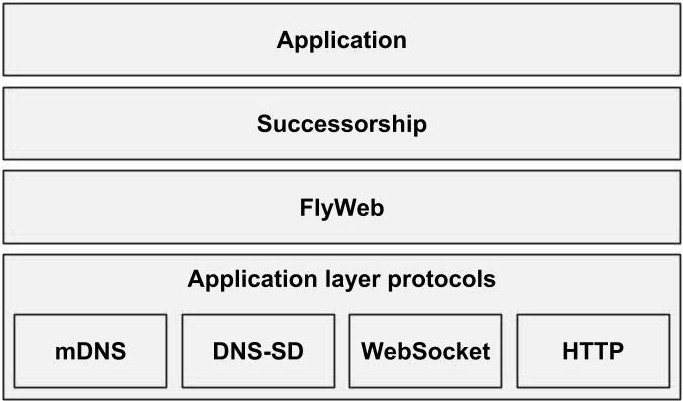
\includegraphics[keepaspectratio,width=6cm]{stack}
    \caption{Successorships Stack}
    \label{fig:stack}
\end{figure}

\noindent\textbf{Roles and shared state.} When a Shippy app is loaded in the browser the new node becomes either a client or server node. 
If it becomes a server node, it becomes a client node to ``itself'' shortly after. 
The application's global state is replicated and shared among all client nodes (see section~\ref{sub:approach_replication_strategy} for our replication strategy). 
The global state can contain arbitrary application data and global metadata accessible only by the \APIshort library. 
One such required metadata field is a \texttt{successors} list containing a list of current clients, except the client node that is currently also the server. 
This list is used to determine which node should become the next server node upon failure of the current one. 
Figure~\ref{fig:roles} depicts the distribution of roles. Node \textit{A} is currently the server with nodes \textit{B...n} being clients. 
Both server and clients have their own replica of the state, accessible through the global state.

\begin{figure}[h]
    \centering
    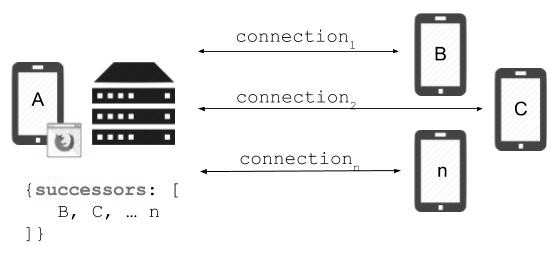
\includegraphics[keepaspectratio,width=6cm]{roles}
    \caption{Successorships Roles}
    \label{fig:roles}
\end{figure}

\noindent\textbf{Service discovery.} 
The \APIshort library comes with a compulsory Firefox add-on responsible for notifying apps with the current set of available \APIshort services. 
In the add-on, we register an event listener to the FlyWeb \textit{DNS-SD} component, which dispatches a list of current local services in frequent intervals.
We sample these events to a maximum frequency of 100ms\footnote{We observed many duplicate and overly frequent event triggers from the \texttt{FlyWebDiscoveryManager} making this sampling necessary.} and filter out all services that were not published in the FlyWeb context. 
We then dispatch our own events containing the current list of FlyWeb services with the service name, IP address and port on the Browser's global \texttt{window} object\footnote{There are a few limitations in this approach that we address in section~\ref{sec:limitations_and_future_work}.}. 
These events are then accessible by event listeners in \APIshort apps as illustrated in listing~\ref{lst:service_discovery}.

\begin{lstlisting}[caption={Event listener for service discovery},label={lst:service_discovery}]
window.addEventListener('flywebServicesChanged', function(event) {
    let services = event.detail.services;
    // e.g. [{ serviceName: "QueueApp",
    // serviceUrl: "http://206.12.69.249:51629" }]
});
\end{lstlisting}

\noindent\textbf{Service publication.}
A \APIshort node will publish a service and hereby become a server node in certain cases depending on service discovery events and the current list of successors in the shared state. 
The decision of whether to become a server is first triggered when (1) \textit{the app is loaded} in the browser and there is currently \textit{no service discovered with the app's name}. 
This decision is then repeated (2) any time a \textit{discovery event} occurs and there is \textit{no such service}\footnote{There is one additional requirement to trigger the decision of whether to publish a service when an event reveals there is currently no service for the app: it must have been connected to a server node previously and been disconnected afterwards. 
If this is not the case, the event should not trigger a server publish as this is handled by the first trigger (app load).}. 
In both cases, the node will become a server if \textit{either} of the following conditions is true:
\begin{itemize}
    \item The \texttt{successors} list is empty \textit{and} this node loaded the application initially\footnote{This is determined by whether the application is currently served by a FlyWeb server node or by other means, e.g. a Web application or a simple HTML file from the file system.}.
    \item The \texttt{successors} list is not empty \textit{and} the first item in the list refers to this client.
\end{itemize}

If one of the above conditions is met in a decision phase, a service with the app's name will be published and that node will become a server. This will then result in a service advertisement  in the local network using the \textit{mDNS} protocol. 

% Figure~\ref{fig:server} illustrates this behavior.

% \begin{figure}[h]
%     \centering
%     
\includegraphics[keepaspectratio,width=8cm]{server}
%     \caption{Successorships service publication}
%     \label{fig:server}
% \end{figure}


\noindent\textbf{Client connection.}
A \APIshort node will become a client when it discovers a service and connects to it.
To do so, \textit{there must be a \APIshort service running with the app's name} and \textit{the node must be currently disconnected}. 
When a node becomes a client, it establishes a \textit{WebSocket} connection to the current server as the first part of the initial handshake. 
On the server side, a unique ID is created for the new client and appended to the \texttt{successors} list. 
The updated \texttt{successors} list is then broadcasted to all currently connected clients. 
The created ID is sent to the new client as the second part of the handshake.
The client node then saves its ID such that it can be matched against the IDs in the \texttt{successors} list in failure scenarios.

\noindent\textbf{Client succession.} 
Whenever the current server fails, a successor must be appointed. 
To determine the successor, clients match their ID against the elements in the \texttt{successors} list.
If their ID matches the first element, this client will become a server node.
Otherwise, it will wait for the new server and connect to it as client.
Referring to the scenario in Figure~\ref{fig:roles}, suppose that server \texttt{A} fails. 
The connected clients \texttt{B} to \texttt{n} detect that failure and match their ID against the ones in the \texttt{successors} list, as presented in Figure~\ref{fig:succession}. Node \texttt{B} will become a server node as its ID matches the first element in the list while other nodes will wait and connect to \texttt{B} as clients nodes.

\begin{figure}[h]
    \centering
    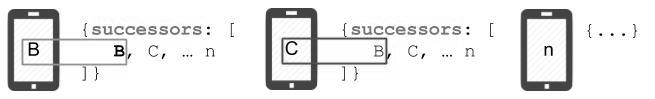
\includegraphics[keepaspectratio,width=6cm]{succession}
    \caption{Successorships client succession}
    \label{fig:succession}
\end{figure}

\noindent\textbf{Server implementation.}
We built on the concept of in-browser Web servers based on the \texttt{navigator.publishServer} implementation in FlyWeb\footnote{https://github.com/flyweb/spec}.
This implementation provides an API for received \textit{HTTP GET} requests and \textit{WebSocket} messages.
Since any Web application relies on static resources (e.g. js, css, images) our FlyWeb server implementation must be able to load and serve these resources when requested by clients.
The documentation of FlyWeb\footnote{https://flyweb.github.io/posts/2016/11/01/introducing-flyweb.html, accessed 2017-12-09} describes that this can be achieved using the browser's \textit{Fetch API}\footnote{https://developer.mozilla.org/en-US/docs/Web/API/Fetch\_API, accessed 2017-12-09}.
However, this is essentially just a redirect to the Web app that served the FlyWeb app at the first place.
Since, after a server failure, the original Web app and its static resources will not be available to clients that took over the server role from another node, \APIshort must store static resources at every node\footnote{Also, we want to support scenarios where only the first client has access to the original Web app that bootstraps the FlyWeb application and clients subsequently only need access to the node that became the first FlyWeb server.}.
We solved this problem by storing all resources required for the \APIshort app in the browser's \texttt{sessionStorage}\footnote{https://developer.mozilla.org/de/docs/Web/API/Window/sessionStorage, accessed 2017-12-09.} that is persistent for the duration of the current browser session.
In the current implementation, all resources obtained upon load of the app are scanned for referenced resources.
These are then fetched and stored in \texttt{sessionStorage}.
Subsequently, when \APIshort request static resources, these can be simply obtained from \texttt{sessionStorage} and served without any access to the original Web app.



% using the \texttt{window.navigator.publishServer} method provided by FlyWeb\footnote{https://github.com/flyweb/spec}. 

\subsection{Replication Strategy and Consistency Guarantees}
\label{sub:approach_replication_strategy}

\textbf{State replication.}
All \APIshort nodes share a versioned global state during the lifetime of the app.
The app is ``alive'' as long as there is one node that advertises the app's service in the local network.
Each time the state is changed on the server node, the state's version is incremented.
The current state is obtained initially by clients triggered by the first handshake with the current server: whenever a new client connects, a WebSocket \texttt{open} event is triggered on the server and a new unique client ID is added to the \texttt{successors} list in the global state object.
The changed state is then broadcasted to all clients\footnote{Note that we are broadcasting the full state in this case rather than a single operation.
A possibly better solution could be that we broadcast only a \texttt{successoradded} operation to all clients except the new one and include the full state for the new client in the \texttt{welcome} message along with the newly created client ID. We come back to this problem in section~\ref{sec:limitations_and_future_work}.}, including the new one.
This ensures that any new client is up-to-date shortly after connecting and that all other clients will have the new client in their \texttt{successors} list.
After a client is connected, it can invoke state changes on the server by calling \texttt{Shippy.call} which will result in a WebSocket message to the server where the submitted operation is applied.
After an operation was applied on the server, this operation is broadcasted to all clients in the order as they appear in the \texttt{successors} list in the shared state.

Since the state is always changed on the current server first and changes are then broadcasted to clients, clients can simply apply the changes locally in ordinary cases.
However, there can be exceptions in certain failure scenarios due to race conditions and the asynchronous nature of WebSocket broadcasting.
We cope with such failures by versioning the state: when clients receive state changes (by listening to \texttt{stateupdate} events), they will check the version of the server's current state and compare it with the version of their local state.
In case their local state is newer than the server state, they will send a \texttt{\_aheadofserver}\footnote{We precede messages not associated with app-defined operations with an underscore.} message to the server with their current local state as payload.
The server can then accept this newer state and again broadcast a state update.
Note that even if several clients send \texttt{\_aheadofserver} messages, the server will only accept these if their state's version is higher than its own, which indicates that consensus will be reached eventually.
In the current \APIshort implementation, we consider clients being ``ahead'' of the server a hypothetical scenario that we could not produce in any of our evaluated use-cases.


\textbf{Reaching consensus.}
We leverage the concepts of \textit{eventual consistency} and \textit{lazy replication} in Shippy \cite{Ladin:1990,Ladin:1992}.
Briefly, this means that nodes holding replicas of the state periodically exchange information, tolerating out-of-sync periods; thus, state may diverge across nodes, but is guaranteed to converge when the system quiesces for some period of time.

We argue that our domain of local ad-hoc offline Web applications will mostly tolerate minor time frames of inconsistent states and we therefore focus on availability and performance rather than accepting the overhead induced by stronger consistency principles.
With the replication strategy previously described, the state manipulation can only happen on the current server and clients are only notified of changes applied on the server.
The most obvious source for inconsistencies would be lost messages carrying operations from server to client and vice versa.
However, this potential problem is mostly mitigated by the design of the WebSocket protocol: each client is connected to the server with a stable bi-directional channel. 
Whenever this channel is interrupted, an \texttt{error} or \texttt{close} event will be triggered on both the client and the server side of the channel.
In such cases, the server will simply remove the client both from its maintained collection of WebSocket clients and the \texttt{successors} list on the shared state (resulting in a \texttt{stateupdate} broadcast). 
The client on the other hand, will try to create a new connection to the server, which will then result in obtaining a fresh copy of the server state.
While we are certain that all nodes will eventually converge to a consistent state with our approach in most scenarios, we cannot eliminate the risk of inconsistencies in certain edge cases (see section~\ref{sec:limitations_and_future_work}).

\subsection{Handled Failure Scenarios}
\label{sub:approach_handled_failure_scenarios}

With our replication and consistency strategies, we handle different scenarios of failures gracefully. There are further scenarios that represent edge cases that we do not cope with at the moment. 
We address these in section~\ref{sec:limitations_and_future_work}.

\textbf{Client disconnection.} 
While disconnecting clients are mostly a trivial circumstance in traditional Web apps, they are more complex in \APIshort apps because the system relies on clients being represented in the shared \texttt{successors} list. 
A disconnecting client will trigger a \texttt{close} event on the current server for the associated WebSocket channel and the disconnected client's ID is obtained. 
The ID is then removed from the \texttt{successors} list on the shared state and the update is broadcasted. 
If the disconnected client was the first element in the \texttt{successors} list, the list will be shifted and the second element will be the new successor.

\textbf{Server disconnection.} 
A disconnected server will result in a WebSocket \texttt{close} event triggered at each connected client. 
After some time, the service discovery mechanism described in Section~\ref{sub:approach_conceptual_description} will reveal that there is no more service currently registered with the app's service name. 
This is the time when one of the previously connected client nodes will become the next server\footnote{We considered starting the next server immediately subsequent to a WebSocket close event but restrained from this approach, considering it too error-prone. For example, a simple page reload on the current server would trigger a WebSocket \texttt{close} event on all clients and one of them immediately becoming the next server. This would introduce another race condition between the first successor and the original server that registers itself again immediately after page reload. Our existing approach deals with this problem much more gracefully: the original server will simply remain the server because the set of current services is updated much less frequently. The downside of our approach is a significantly increased time of recovery. See section~\ref{sec:limitations_and_future_work} for further details.}: each client compares the first item in the shared \texttt{successors} list with its ID (obtained with the \texttt{welcome} message of the initial handshake). 
If it matches, the client will publish a server as described in Section~\ref{sub:approach_conceptual_description}. 
Otherwise, it will continue listening for service discovery events until a service with the app's name is available and connect to it.

\textbf{Simultaneous disconnection.} 
In this scenario, the server and one or multiple clients fail within a short time frame. 
For example, both the server and the first successor could disconnect and other clients would not receive the update that the first successor disconnected. 
If we did not target this case specifically, no client would become the new server because they all expect a disconnected client to do so. 
We solve this problem with a \textit{repeated timer} algorithm: clients that are not the first item in the \texttt{successor} list set a timer that will prune the first item from the list after some time. 
This interval is set sufficiently to give the current first successor enough time to publish the service. 
The interval is varied with a random number to make it highly unlikely that two clients prune successors at about the same time which could result in race conditions publishing a service. 
At some point in this process, one other client will be the first in the \texttt{successors} list and will become a server. 
Other clients will be notified eventually by a service discovery event and connect to the new server.

\section{Evaluation}
\label{sec:evaluation}

\section{Limitations and Future Work}
\label{sec:limitations_and_future_work}


% ===
% Felix: below is just a random collection of notes I took during writing other parts

% LIMITATIONS:
% all services are published to web apps
% ip + port => no hostnames
% only mac
% time to recovery
% weak consistency
% server: prevent second fetch 

% LIMITATION
% sometimes broadcast whole state
% async state updates => could wait for first succ's ack

%In the current implementation, the full state is broadcasted when a new client connects. This could be improved in the future by broadcasting only a 

% LIMITATIONS
%In certain failure cases where a client state is newer than a server state, clients can essentially \textit{overwrite} the server state.
%This opens up the risk of being spoofed by malicious clients imposing a manipulated state onto our network, but as stated previously, we allow ourselves to assume full trust between all participants in the network.
%We have considered using a \textit{CRDT} for our implementation, but we believe that the constraint of commutativity of operations, or associativity of merging conflicting states, is potentially too restricting for the range of applications we would want to allow to run on our framework.
%We have also considered to notify the first client in the \texttt{successors} list and only broadcast to other clients when an acknowledgement was received.
%We faced technical difficulties with this strategy and were not convinced enough of the benefits to justify further efforts.

% LIMITATIONS
% transmission queue

% We considered starting the next server immediately subsequent to a WebSocket close event, but restrained from this approach being too error-prone. For example, a simple page reload on the current server would trigger a WebSocket \texttt{close} event on all clients and one of them immediately becoming the next server. This would introduce another race condition between the first successor and the original server that registers itself again immediately after page reload. Our existing approach deals with this problem much more gracefully: the original server will simply remain the server because the set of current services is updated only in much longer intervals. The downside of our approach is a significantly increased time of recovery.

\section{Related Work}
\label{sec:related_work}

\textbf{Zeroconf.}
Several researchers propose have investigated Zeroconf~\cite{Gunes2002, Bohnenkamp2003, Jara:2012:IPv6DNS-SD}.
For instance, \cite{hong2007accelerating} discusses that Zeroconf service discovery may cause overheads to the network while discovering new services.
Thus, proposing an algorithm to accelerate service discovery based on network topology changes.
Since a server failure would imply a change in the network topology, i.e. the server node being removed from the topology, 
client nodes our implementation could use their approach to accelerate service discovery. 
Nonetheless, their implementation used a LINUX Wireless extensions, which may not be accessible within a browser.
Thus, we used the FlyWeb service discovery implementation.

In~\cite{stolikj2016context}, Stolikj et al. argue that the number of published services in a network may also slow down service discovery.
As a solution, they propose a context based approach, where queries specify which services they are interested in.
This context based approach is highly suitable for our work and we could use it to filter \APIshort services.
However, their approach changes service discovery queries and we question whether this could be easily integrated with existing devices.


\textbf{Zeroconf.}



\section{Conclusion}
\label{sec:conclusion}

As networking capabilities become more ubiquitous across different types of devices, applications that communicate over local area networks become more common.
Using a proper suite of networking protocols and technologies, these applications can discover other devices in the network and exchange data with them.
One appealing way to build such apps is using zeroconf networks and web browsers.
Nonetheless, applications operating in zeroconf still face normal challenges imposed by the type of network that they operate on, e.g. 
unstable wireless links or host mobility. Also, developers have little to no browser API support for these technologies.


To address the aforementioned issues, we proposed \APINameNoSpace, which abstracts and decouples zeroconf logic from the application logic and seamlessly integrates fault-tolerance to applications that require a state but face failures due to intermittent connectivity. We evaluated \APIName by measuring network traffic and state recovery in face of failures in proof of concept applications. \APIName supports all its intended use cases and future work will improve bottlenecks identified during our evaluation.


\bibliographystyle{abbrv}
\bibliography{flyweb_paper}

\end{document}

